% =====================================================================
%  Attention-Allocated Retrieval
%
%  Water-filling attention allocation (T2 of the split-attention paper)
%  assumes the environment has diminishing returns. Federated joins do
%  not, below a threshold that is computable in closed form from corpus
%  size alone. The threshold flips the optimal policy rather than
%  bounding lost optimality, so the allocator must gate --- and refuse.
% =====================================================================
\documentclass[11pt,twocolumn,a4paper]{article}

\usepackage[utf8]{inputenc}
\usepackage[T1]{fontenc}
\usepackage{lmodern}
\usepackage[a4paper,margin=2.4cm]{geometry}
\usepackage{amsmath,amssymb,amsthm,mathtools}
\usepackage{bm}
\usepackage{booktabs}
\usepackage{array}
\usepackage{enumitem}
\usepackage{microtype}
\usepackage{xcolor}
\usepackage{graphicx}
\usepackage{listings}
\usepackage[round,sort&compress]{natbib}
\usepackage[colorlinks=true,linkcolor=blue!45!black,
            citecolor=blue!45!black,urlcolor=blue!45!black]{hyperref}
\usepackage{cleveref}

% ---- Theorem-like environments ----
\newtheoremstyle{thmstyle}{\topsep}{\topsep}{\itshape}{}{\bfseries}{.}{.5em}{}
\theoremstyle{thmstyle}
\newtheorem{theorem}{Theorem}[section]
\newtheorem{lemma}[theorem]{Lemma}
\newtheorem{proposition}[theorem]{Proposition}
\newtheorem{corollary}[theorem]{Corollary}
\theoremstyle{definition}
\newtheorem{definition}[theorem]{Definition}
\newtheorem{rulename}[theorem]{Rule}
\newtheorem{principle}[theorem]{Principle}
\newtheorem{example}[theorem]{Example}
\theoremstyle{remark}
\newtheorem{remark}[theorem]{Remark}
\newtheorem{notation}[theorem]{Notation}

\crefname{principle}{Principle}{Principles}
\Crefname{principle}{Principle}{Principles}

% ---- listing style for the allocator interface ----
\definecolor{kw}{RGB}{30,64,175}
\definecolor{cmt}{RGB}{22,101,52}
\definecolor{strc}{RGB}{159,18,57}
\definecolor{lstbg}{RGB}{250,250,250}
\lstset{
  language=Python,
  basicstyle=\ttfamily\small,
  keywordstyle=\color{kw}\bfseries,
  commentstyle=\color{cmt}\itshape,
  stringstyle=\color{strc},
  backgroundcolor=\color{lstbg},
  frame=single,framesep=4pt,xleftmargin=6pt,xrightmargin=4pt,
  breaklines=true,showstringspaces=false,columns=fullflexible,tabsize=2
}

% ---- shorthand ----
\newcommand{\R}{\mathbb{R}}
\newcommand{\N}{\mathbb{N}}
\newcommand{\E}{\mathbb{E}}
\newcommand{\eff}{e}
\newcommand{\estar}{e^{*}}
\newcommand{\ucross}{u^{\dagger}}
\newcommand{\abs}[1]{\lvert#1\rvert}
\newcommand{\shk}[1]{\texttt{#1}}
\newcommand{\yield}{Y}

\title{\textbf{On the Optimality of Attention-Allocated Retrieval:\\[3pt]
Computable Thresholds of Federated Retrieval Pipelines}}

\author{%
Kundai Farai Sachikonye\\
\small Technical University of Munich\\
\small AIMe Registry for Artificial Intelligence\\
\small \texttt{kundai.sachikonye@wzw.tum.de}}

\date{\today}

\begin{document}
\maketitle

% =====================================================================
\begin{abstract}
\noindent
Water-filling attention allocation---theorem T2 of the split-attention
agent framework \citep{sachikonye2026splitattention}---is optimal under a
diminishing-returns assumption which that paper is careful to flag as a
property of the \emph{environment} rather than of the allocator. This
paper measures the assumption in one environment that matters: a
federated retrieval pipeline that must join records across endpoints
before a reasoner can be invoked over them
\citep{doerr2025limits,sachikonye2026tacat}. The assumption is false, and
it fails in a way that is exactly characterised.

Expected join yield after $\eff$ queries is
$\yield(\eff)=N p^{2}$ with $p=1-(1-1/N)^{\eff/2}$, because a join
requires \emph{both} sides of a pair to have been drawn. Squaring a
saturating function gives a sigmoid, so retrieval has \emph{increasing}
returns early. We show (i)~the inflection is exact,
$\estar=2\ln 2/\ln\!\big(1/(1-1/N)\big)\to 2N\ln 2$, and the yield there
is $N/4$---\emph{exactly a quarter of the joinable corpus for every $N$},
so the threshold is computable at run time from a count query with no
fitted constant (\Cref{thm:threshold}); (ii)~the threshold \emph{reverses
the optimal policy} rather than bounding lost optimality: below $\estar$
the optimum is at a corner and committing the whole budget to one join
beats spreading it by up to $97\%$, while above $\estar$ the ordering
reverses and the even split wins (\Cref{thm:reversal}); and (iii)~the
optimum equalises effort measured in units of each join's \emph{own}
threshold, $\eff/\estar$, not raw effort---which is what makes a single
shadow price meaningful across corpora of different sizes
(\Cref{prop:normalised}).

We then build the allocator these results dictate and check it against
exhaustive search over the simplex, with which it shares no reasoning.
It agrees to within $0.0000\%$ at two sources and $10^{-6}$ at three, and
below threshold it \emph{refuses}: it declines to allocate and names the
budget at which it could, a refusal of the same shape as the two the
medium-vertex paper derives from the medium
\citep{sachikonye2026medium}, but with a threshold computable from corpus
size rather than fitted. Twenty-one checks pass, six of them negative
controls that must fail on well-formed input.

We report two of our own measurement errors and one genuine flaw in the
allocator, because each is load-bearing. The first two made the finding
look like an artefact---Monte Carlo noise five times the true curvature,
then a parity artefact---and were settled only by evaluating the closed
form with no sampling at all. The third is more instructive:
$\text{budget}\ge\sum_i\estar_i$ is \emph{necessary but not sufficient}
for the interior solution to be optimal, and an allocator built on that
false sufficiency loses $8\%$ at the boundary. No self-consistency check
could have caught it; only the brute-force comparison did.
\end{abstract}

\noindent\textbf{Keywords:} attention allocation; water-filling;
diminishing returns; federated query; convexity threshold; corner
solution; shadow price; refusal; negative control; knowledge graph
retrieval.

\tableofcontents

% =====================================================================
\section{Introduction}
\label{sec:intro}
% =====================================================================

\subsection{An assumption flagged and not tested}

The split-attention agent framework gives an agent a finite attention
budget and a rule for spending it \citep{sachikonye2026splitattention}.
Theorem T2 establishes that the optimal spend equalises marginal return
across activities---water-filling, the same rule that allocates power
across parallel channels \citep{cover2006elements} and, more generally,
any separable resource under a concave objective
\citep{boyd2004convex}. Its hypothesis is that each activity's return is
concave in the effort spent on it.

That paper is explicit that concavity is an assumption about the
\emph{environment}, not a structural property of the allocator. It is
stated, used, and---in the setting it was written for---plausible. The
honest thing to do with a flagged assumption is to measure it somewhere
it matters.

The setting we measure it in is retrieval. A pipeline of the kind
described by \citet{doerr2025limits} invokes a reasoner at run time over
records gathered from several endpoints. Before the reasoner can run,
the records must be there; gathering them costs queries; the query budget
is finite. This is an attention-allocation problem in the exact sense T2
addresses, with sources in place of activities and queries in place of
attention. If T2 applies, the agent has a rule. If it does not, the agent
needs to know that before it acts.

\subsection{Why joins are the case that matters}
\label{sec:whyjoins}

Not all retrieval is alike, and the difference is not stylistic.

Retrieving \emph{distinct entities} from a single endpoint is
coupon-collecting: after $\eff$ draws the expected coverage is
$N\big(1-(1-1/N)^{\eff}\big)$, which is concave everywhere
\citep{motwani1995randomized,feller1968probability}. T2 applies without
qualification.

Retrieving \emph{paginated} results returns a fixed number of new records
per query until the source is exhausted. Marginal yield is constant, not
decreasing, so T2's hypothesis fails---but harmlessly, in the sense that
a linear objective's optimum is also at a corner and any allocation
achieves the same total.

Retrieving a \emph{federated join} is different in kind. A joined record
exists only when \emph{both} sides of the pair have been drawn. If each
side is drawn independently with the same effort, the expected number of
completed joins goes as the \emph{square} of a coverage probability. This
is the regime the pipelines in question actually operate in: Rhea joined
to UniProt, ChEBI joined to Rhea
\citep{bansal2022rhea,hastings2016chebi,uniprot2023,buil2013federated}.
It is also, as we show, the one regime of the three where T2's failure
changes what the agent should do.

\subsection{What we prove}
\label{sec:contributions}

\begin{enumerate}[leftmargin=1.4em,itemsep=3pt]
\item \textbf{The join yield surface is a sigmoid, and its inflection is
exact.} $\yield(\eff)=Np^{2}$ with $p=1-(1-1/N)^{\eff/2}$ is convex below
$\estar=2\ln2/\ln\!\big(1/(1-1/N)\big)$ and concave above, with
$\estar\to 2N\ln2$ and $\yield(\estar)=N/4$ for every $N$
(\Cref{thm:threshold}). The threshold needs one number the pipeline
already has.

\item \textbf{The threshold reverses the optimal policy.} Below $\estar$
the optimum is at a corner---not near one---and committing beats
spreading by at least $17.9\%$ over the sampled range and by $97\%$ at
the smallest budgets. Above $\estar$ the ordering reverses
(\Cref{thm:reversal}). A gate is therefore not a refinement; without one
the allocator picks the worse of the two available actions, and does so
most severely for the agents with the least budget.

\item \textbf{The state variable is normalised effort.} The optimum
equalises $\eff/\estar$ across joins, not $\eff$
(\Cref{prop:normalised}). With corpora of $30$ and $90$ the optimum gives
$2.00\,\estar$ and $1.98\,\estar$ while the raw efforts differ
threefold.

\item \textbf{The allocator refuses.} Below every threshold no
allocation rule available to it is well-founded, so it declines and
reports the budget that would suffice
(\Cref{def:refuse-allocate,thm:refusal-nonvacuous}). We verify the
refusal fires, that it does \emph{not} fire above threshold, and that the
budget it names actually resolves it.
\end{enumerate}

\subsection{What we do not claim}
\label{sec:notclaim}

We do not claim T2 is wrong. \Cref{thm:threshold} is a \emph{bound}, and
the negative control in \Cref{sec:validation} confirms the concave branch
recovers T2 exactly: above $\estar$ the optimum for two identical joins
is the even split to within $0.0\%$. We do not claim the join model is
the only model of federated retrieval---it assumes independent uniform
draws on both sides, and \Cref{sec:scope} sets out what breaks when that
fails. And we do not claim the allocator is optimal in general; we claim
it agrees with brute force on the cases we checked, and we report the
case where an earlier version did not.

% =====================================================================
\section{The join yield surface}
\label{sec:surface}
% =====================================================================

\subsection{Model}

\begin{definition}[Federated join source]
\label{def:source}
A \emph{join source} is a pair of endpoints together with a set of $N$
\emph{joinable keys}: values of the shared attribute for which a record
exists on both sides. $N$ is not the record count; it is the count of
keys that would survive the join, which is obtainable from a count query
before any retrieval is done.

Spending effort $\eff$ on the source means issuing $\eff$ queries, split
evenly between the two sides, each returning one key drawn uniformly at
random with replacement.
\end{definition}

The replacement assumption is the conservative one: sampling without
replacement would only make coverage rise faster, sharpening every
conclusion below. \Cref{sec:scope} returns to this.

\begin{lemma}[Yield]
\label{lem:yield}
Under \Cref{def:source}, the expected number of completed joins after
effort $\eff$ is
\begin{equation}
\label{eq:yield}
\yield(\eff) \;=\; N\,p(\eff)^{2},
\qquad
p(\eff) \;=\; 1-\Big(1-\tfrac{1}{N}\Big)^{\eff/2}.
\end{equation}
\end{lemma}

\begin{proof}
Each side receives $\eff/2$ draws. For a fixed key, the probability it
is missed on one side after $\eff/2$ uniform draws with replacement is
$(1-1/N)^{\eff/2}$, so it is present with probability $p(\eff)$. The two
sides are drawn independently, so the key is joinable with probability
$p^{2}$. Summing the indicator over all $N$ keys and using linearity of
expectation gives \Cref{eq:yield}; note this requires no independence
\emph{between} keys.
\end{proof}

\Cref{eq:yield} is the whole paper in one line. $p$ is concave. $p^{2}$
is not, because squaring is convex and increasing, and the composition of
a convex increasing function with a concave one is neither in general.
The next result says exactly where each behaviour holds.

\subsection{The threshold}

\begin{theorem}[Convexity threshold and the quarter-corpus law]
\label{thm:threshold}
Let $q=1-1/N$ with $N\ge2$. Then $\yield$ in \Cref{eq:yield} satisfies
\begin{enumerate}[label=(\roman*),leftmargin=1.8em,itemsep=2pt]
\item $\yield''(\eff)>0$ for $\eff<\estar$ and $\yield''(\eff)<0$ for
$\eff>\estar$, where
\begin{equation}
\label{eq:estar}
\estar \;=\; \frac{2\ln 2}{\ln(1/q)};
\end{equation}
\item $\estar \to 2N\ln 2$ as $N\to\infty$, from below;
\item $\yield(\estar) = N/4$ \emph{exactly}, for every $N$.
\end{enumerate}
\end{theorem}

\begin{proof}
Write $r(\eff)=q^{\eff/2}$, so $p=1-r$ and $r'=\tfrac12 r\ln q$. Then
\[
\yield' = 2Np\,(-r') = -N r p \ln q ,
\]
and differentiating again,
\[
\yield'' = -N\ln q\,\big(r'p + r p'\big)
         = -N\ln q\,\big(\tfrac12 r\ln q\,p + r\cdot(-\tfrac12 r \ln q)\big),
\]
which simplifies to
\begin{equation}
\label{eq:secondderiv}
\yield''(\eff) \;=\; -\tfrac{N}{2}(\ln q)^{2}\, r\,\big(p-r\big)
\;=\; \tfrac{N}{2}(\ln q)^{2}\, r\,\big(2r-1\big),
\end{equation}
using $p-r=1-2r$. Since $N>0$, $(\ln q)^{2}>0$ and $r>0$, the sign of
$\yield''$ is the sign of $2r-1$. Thus $\yield''>0$ exactly when
$r>\tfrac12$, i.e.\ $p<\tfrac12$, and $\yield''<0$ exactly when
$p>\tfrac12$. Solving $r(\eff)=\tfrac12$ gives
$q^{\eff/2}=\tfrac12$, hence $\eff=2\ln2/\ln(1/q)$, which is
\Cref{eq:estar}. This proves (i).

For (ii), $\ln(1/q)=-\ln(1-1/N)=1/N+1/(2N^{2})+O(N^{-3})$, so
$\estar = 2N\ln2\big(1+\tfrac{1}{2N}+O(N^{-2})\big)^{-1}
        = 2N\ln 2 - \ln 2 + O(N^{-1})$,
approaching $2N\ln2$ from below.

For (iii), at $\eff=\estar$ we have $r=\tfrac12$ hence $p=\tfrac12$,
so $\yield=Np^{2}=N/4$ identically in $N$.
\end{proof}

\begin{remark}[Why (iii) is the useful part]
\label{rem:quarter}
Parts (i) and (ii) locate the threshold in units of effort, which an
agent can compute but cannot easily interpret. Part (iii) states it in
units of \emph{result}: the threshold is precisely the point at which a
quarter of the joinable corpus has been recovered. This holds exactly,
for every $N$, with no asymptotics. An agent that has retrieved fewer
than $N/4$ joins is below threshold; one that has retrieved more is
above. The test requires no fitted constant and no calibration, and it
can be evaluated on results already in hand rather than on a model of
effort.
\end{remark}

\begin{corollary}[The convexity is structural]
\label{cor:structural}
The sign change in \Cref{eq:secondderiv} depends on $N$ only through the
positive factor $\tfrac{N}{2}(\ln q)^{2}$. No choice of corpus size, and
no amount of sampling, removes the convex branch.
\end{corollary}

\Cref{cor:structural} is stated because we needed it. Two earlier
attempts to observe the convexity from simulation failed for reasons
that had nothing to do with the physics
(\Cref{sec:ourerrors}), and only evaluation of the closed form settled
the matter.

\begin{figure*}[!htbp]
    \centering
    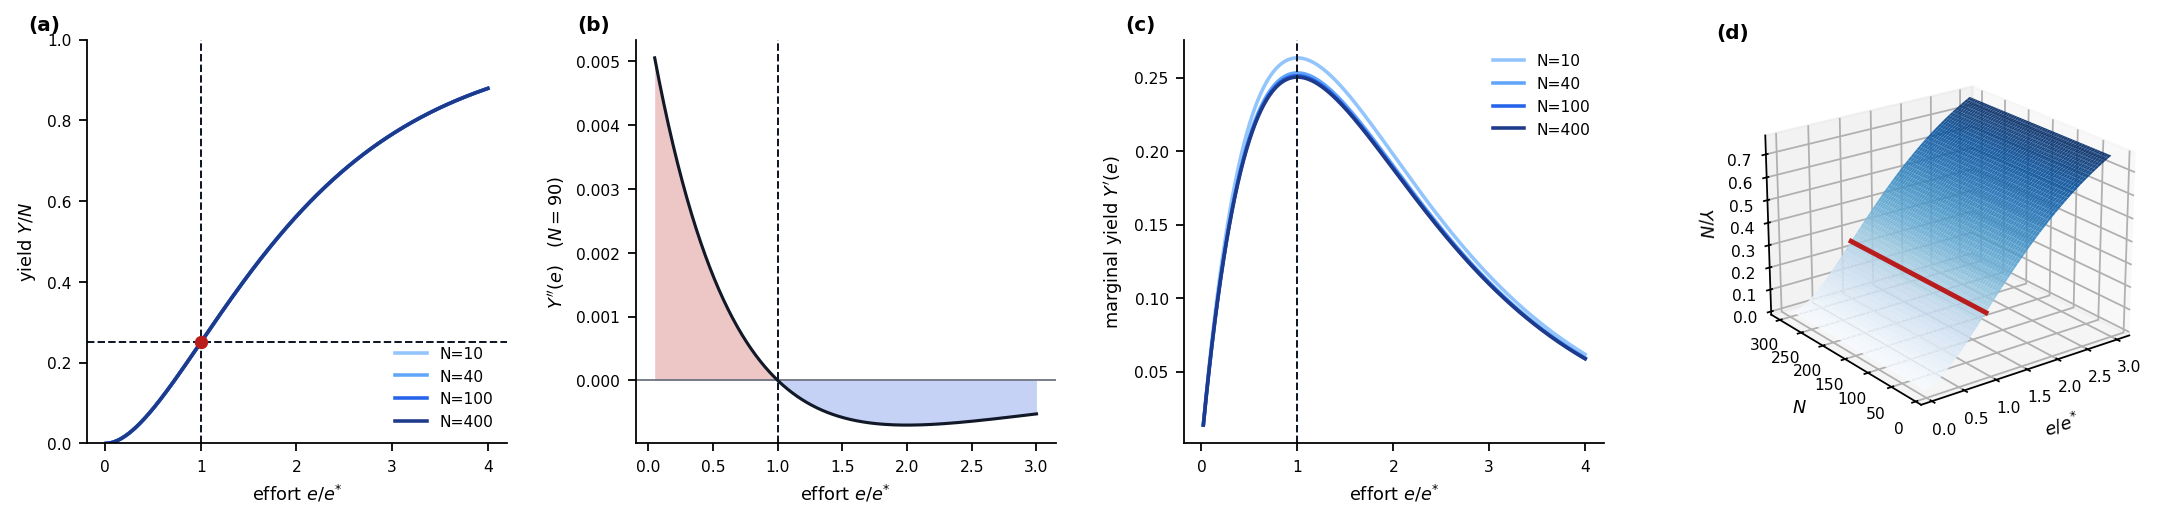
\includegraphics[width=\textwidth]{figures/panel_01_yield_surface.png}
    \caption{\textbf{The Federated-Join Yield Surface and Its Inflection.}
    (\textbf{A})~Normalised yield $Y(e)/N$ for corpus sizes $N \in \{10, 40, 100, 400\}$ against effort measured in units of each corpus's own threshold $e^{*}$. The four curves are drawn from $Y(e) = Np^2$ with $p = 1 - (1 - 1/N)^{e/2}$; because $p$ saturates and squaring a saturating function does not, every curve is sigmoid rather than concave. All four cross $Y/N = 0.25$ at exactly $e/e^{*} = 1$ (red marker), which is the quarter-corpus law: the yield at the inflection is $N/4$ for every $N$, with no asymptotics and no fitted constant.
    (\textbf{B})~Second derivative $Y''(e) = \tfrac{N}{2}(\ln q)^2 r(2r - 1)$, where $q = 1 - 1/N$ and $r = q^{e/2}$, evaluated at $N = 90$ ($e^{*} = 124.07$). The convex region $Y'' > 0$ is shaded red and the concave region $Y'' < 0$ blue. The sign change occurs at $e/e^{*} = 1$ and nowhere else, so the domain splits into exactly two branches: increasing returns below threshold, diminishing returns above it.
    (\textbf{C})~Marginal yield $Y'(e) = -Nrp\ln q$ for the same four corpora. Marginal yield does not decrease monotonically---it \emph{rises} to a peak at $e/e^{*} = 1$ before falling. This peak is the mechanism behind the necessary-versus-sufficient failure: at a budget just above $\sum_i e^{*}_i$ every source sits barely onto its concave branch where its marginal return is still near maximal, so withdrawing one source outright can free enough budget to push another further up its curve.
    (\textbf{D})~Yield surface $Y/N$ over $(e/e^{*},\,N)$ for $N \in [10, 300]$, with the threshold ridge $e = e^{*}(N)$ traced in red at constant height $0.25$. The ridge is flat in $N$: the inflection sits at the same normalised effort and the same fractional yield for every corpus size, which is why $e/e^{*}$ and not $e$ is the allocator's state variable.}
    \label{fig:panel1}
\end{figure*}

% ---------------------------------------------------------------------

% ---------------------------------------------------------------------

% =====================================================================
\section{The threshold reverses the optimal policy}
\label{sec:reversal}
% =====================================================================

That an objective is non-concave on part of its domain does not by itself
mean an allocator built for concave objectives is dangerous there. It
might merely be suboptimal by a controllable amount. This section shows
it is not: below the threshold the water-filling answer and the optimal
answer are on opposite sides of the decision.

\subsection{Corner versus interior}

\begin{theorem}[Policy reversal]
\label{thm:reversal}
Consider two join sources with the same corpus size $N$ and a shared
budget $B$, allocated as $(x, B-x)$ with $x\in[0,B]$. Write
$u=B/\estar$. There is a single crossover
\begin{equation}
\ucross \;=\; 2\log_2\!\bigl(1+\sqrt2\,\bigr)\;=\;2.5431\ldots,
\label{eq:ucross}
\end{equation}
the same for every $N$ and not merely in the limit, such that:
\begin{enumerate}[label=(\alph*),leftmargin=1.8em,itemsep=2pt]
\item If $u<\ucross$, committing the entire budget to one source is
optimal, and the optimum is the endpoint $x=0$ (or $x=B$).
\item If $u>\ucross$, the symmetric split $x=B/2$ is optimal.
\item At $u=\ucross$ the two policies have exactly equal yield.
\end{enumerate}
In particular the optimum jumps from $x/B=0$ to $x/B=1/2$
discontinuously: no asymmetric interior split is ever optimal.
\end{theorem}

\begin{proof}
Work in normalised effort. Write $q=1-1/N$ and $t=q^{\,B/2}$; since
$q^{\estar/2}=\tfrac12$ by the definition of $\estar$, we have exactly
$t=2^{-u/2}$ for every $N$, with no approximation. The commit policy
then yields $N(1-t^{2})^{2}$ and the even split $2N(1-t)^{2}$. Setting
these equal,
\begin{equation*}
(1-t)^{2}(1+t)^{2}\;=\;2(1-t)^{2},
\end{equation*}
and since $t<1$ we may divide by $(1-t)^{2}$ to get $(1+t)^{2}=2$, hence
$t=\sqrt2-1$ and $u=-2\log_2(\sqrt2-1)=2\log_2(1+\sqrt2)$, which is
\eqref{eq:ucross}. This is the unique crossing, because
$(1-t^{2})^{2}-2(1-t)^{2}=(1-t)^{2}\bigl[(1+t)^{2}-2\bigr]$ changes sign
only where $(1+t)^{2}=2$; as $t$ is strictly decreasing in $u$, the
commit policy wins below $\ucross$ and loses above it.

For the stronger statement that these two are the only candidates: when
$u<1$ every feasible $x$ leaves both sources on the convex branch, so
the total is convex and attains its maximum at an extreme point
\citep{gale1989corner,boyd2004convex}. When $u\ge2$ the total is concave
on $x\in[\estar,B-\estar]$, so $x=B/2$ is the best \emph{interior}
point---but concavity there says nothing about $x\notin[\estar,B-\estar]$,
and the endpoints lie outside it. The comparison above is what settles
those, and it is why the crossover is at $\ucross$ rather than at the
edge $u=2$ of the concave region.
\end{proof}

\begin{figure*}[!htbp]
    \centering
    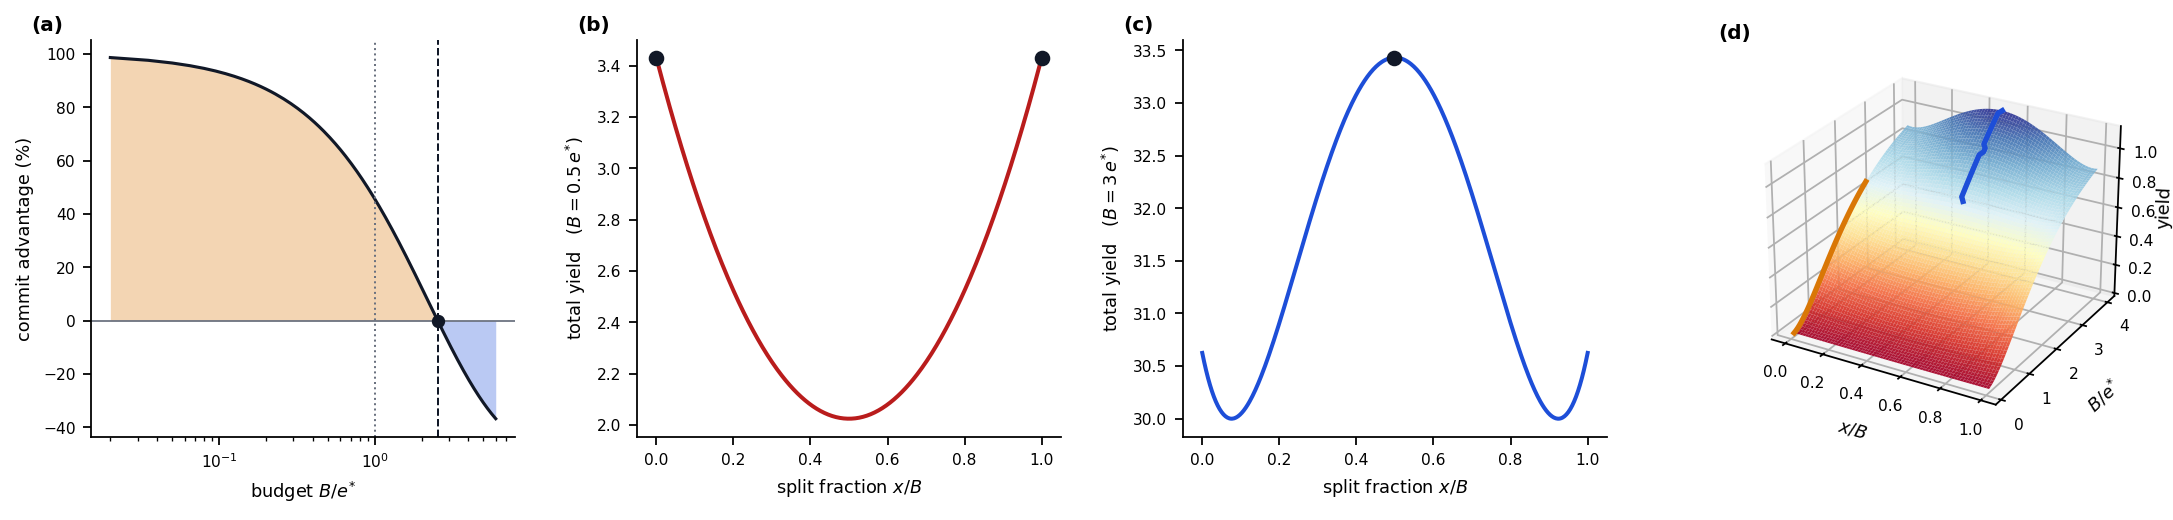
\includegraphics[width=\textwidth]{figures/panel_02_policy_reversal.png}
    \caption{\textbf{The Threshold Reverses Which Allocation Policy Is Optimal.}
    (\textbf{A})~Relative advantage of committing the whole budget to one source over splitting it evenly, against budget $B/e^{*}$ on a logarithmic axis, for two sources of equal corpus size $N = 40$. Committing wins by $98.6\%$ at $B = 0.02\,e^{*}$, by $45.7\%$ at $B = e^{*}$, and still by $12.5\%$ at $B = 2e^{*}$ where both sources are already on their concave branches. The advantage crosses zero at $u^{\dagger} = 2\log_2(1 + \sqrt{2}) = 2.5431$ (solid marker), \emph{not} at the dotted line $B = e^{*}$ where the yield curve inflects. The crossing is located by the plotting code rather than drawn at a predicted value, and the gap between $u^{\dagger}$ and the edge of the concave region at $u = 2$ is what falsified an earlier version of the reversal theorem.
    (\textbf{B})~Total yield against split fraction $x/B$ at a sub-threshold budget $B = 0.5\,e^{*}$. The curve is convex and attains its maximum at both endpoints ($3.431$ at $x/B \in \{0, 1\}$) against $2.025$ at the centre---a $69.4\%$ penalty for splitting. The optimum is \emph{at} a corner, not near one.
    (\textbf{C})~The same construction at a super-threshold budget $B = 3e^{*}$. The ordering has reversed: the maximum is the symmetric split ($33.43$ at $x/B = 0.499$) against $30.63$ at the endpoints. Water-filling is exactly right here and exactly wrong in (B).
    (\textbf{D})~Total yield over (split fraction, budget) for two equal corpora, with the ridge of optima traced---orange below the crossover, blue above. The ridge jumps from the boundary $x/B = 0$ to the centre $x/B = 1/2$ with no intermediate values, confirming the discontinuity: no asymmetric interior split is ever optimal, so an allocator cannot reach the answer by tuning a split fraction continuously.}
    \label{fig:panel2}
\end{figure*}

\begin{remark}[Why the boundary is not $2\estar$]
\label{rem:not2estar}
It is tempting to stop at the observation that both sources are on their
concave branches once $B\ge2\estar$, and conclude the symmetric split
wins there. It does not. At $B=2\estar$ exactly, committing yields
$0.5625N$ against the even split's $0.5N$---the corner is still ahead by
$12.5\%$, and stays ahead until $u=\ucross$. Concavity on the interior
region is necessary for the interior optimum, not sufficient for it,
because the competing optima sit on a part of the feasible set where the
function is convex. This is the same necessary-versus-sufficient error
that \Cref{prop:notsufficient} records for the multi-source allocator;
an earlier draft of this theorem asserted the $2\estar$ boundary, and
\Cref{fig:panel2}(a)---whose crossing is computed, not drawn---is what
exposed it.
\end{remark}

\begin{remark}[A second exact constant]
\label{rem:yieldatucross}
Substituting $t=\sqrt2-1$ into either policy gives the common yield at
the crossover in closed form,
\begin{equation}
\yield(\ucross\estar)\;=\;4\bigl(\sqrt2-1\bigr)^{2}N
\;=\;\bigl(12-8\sqrt2\bigr)N\;\approx\;0.68629\,N,
\label{eq:yieldatucross}
\end{equation}
exact for every $N$, as \eqref{eq:ucross} is. It is the companion to the
quarter-corpus law of \Cref{thm:threshold}(iii): $\estar$ is where a
join has recovered a quarter of its corpus, and $\ucross\estar$ is where
it has recovered $12-8\sqrt2$ of it and an allocator's optimal policy
flips. Both are properties of the join surface alone, with no fitted
constant and no dependence on corpus size.
\end{remark}

The empirical content is in the magnitude. Over budgets from $0.15$ to
$0.90$ of $\estar$, committing beats the even split at every budget by
at least $17.9\%$; the worst case measured is a $97\%$ relative loss at
$0.02\,\estar$. The loss grows as the budget shrinks, so the agents with
the least attention---the ones an allocation theory exists to help---are
the ones an ungated allocator hurts most.

\begin{remark}[The optimum is \emph{at} a corner, not near one]
\label{rem:atcorner}
\Cref{thm:reversal}(a) compares two policies, which leaves open that some
third, interior policy beats both. Brute-force search over $2001$ splits
of a budget of $0.50\,\estar$ places the unconstrained optimum at
$x=0$ exactly. There is no interior optimum being missed.

Sweeping the budget rather than fixing it makes the stronger point.
Brute-force argmax over $4001$ splits at
$u\in\{1.0,1.5,2.0,2.2,2.4\}$ returns $x/B=0.000$ at every one; at
$u\in\{2.7,3.0\}$ it returns $x/B=0.500$. The optimal split never takes
an intermediate value---it jumps at $\ucross$. An allocator therefore
cannot approach the correct answer by tuning a split fraction
continuously, which is a second reason the decision must be gated rather
than smoothed.
\end{remark}

\subsection{Normalised effort}

Identical corpora make the reversal easy to state and easy to
under-generalise. The mixed case is where the allocation rule earns its
keep.

\begin{proposition}[The optimum equalises $\eff/\estar$]
\label{prop:normalised}
For sources with corpus sizes $N_i$ and thresholds $\estar_i$, at budgets
where every source is on its concave branch, the optimal allocation
equalises the normalised efforts $u_i=\eff_i/\estar_i$ to first order,
rather than the raw efforts $\eff_i$.
\end{proposition}

\begin{proof}[Argument]
On the concave branch the optimum equalises marginal yields,
$\yield_i'(\eff_i)=\lambda$ for all $i$. From the proof of
\Cref{thm:threshold}, $\yield_i'=-N_i r_i p_i\ln q_i$ where
$r_i=q_i^{\eff_i/2}=2^{-u_i}$ by \Cref{eq:estar}, so $r_i$---and hence
$p_i=1-r_i$---depends on $\eff_i$ \emph{only} through $u_i$. Therefore
$\yield_i'(\eff_i)=N_i\ln(1/q_i)\,\cdot\,2^{-u_i}(1-2^{-u_i})$. Since
$N_i\ln(1/q_i)\to 1$ as $N_i\to\infty$ (from
$\ln(1/q_i)=1/N_i+O(N_i^{-2})$), the prefactor becomes common to all
sources, and equalising $\lambda$ reduces to equalising the function
$u\mapsto 2^{-u}(1-2^{-u})$, hence to equalising $u_i$ on the branch
$u>1$ where it is monotone.
\end{proof}

Measured: with corpora of $30$ and $90$ ($\estar=40.9$ and $124.1$) and a
budget of $327.1$, the optimum allocates $81.9$ and $245.3$---that is,
$2.00\,\estar$ and $1.98\,\estar$, equal to within $1.3\%$, while the raw
efforts differ threefold. At three sources with corpora $20$, $60$, $200$
the normalised efforts are $2.54$, $2.51$, $2.49$, equal to within
$1.7\%$, while raw efforts are $69$, $207$, $690$.

\begin{corollary}[A global threshold is wrong in both directions]
\label{cor:perjoin}
Because $\estar$ depends on $N$, a single budget threshold applied to a
mixed set of sources will gate a large-corpus join as though it were
above threshold when it is below, and vice versa. Gating must be per
source, in normalised units.
\end{corollary}

At the mixed-corpus optimum the small join receives $25.0\%$ of the
budget, yielding $66.971$ against $58.659$ for an even split ($+14.2\%$)
and $63.383$ for committing everything to one source ($+5.7\%$). The
optimum is strictly interior and strictly better than both naive
policies, so neither can imitate it: the rule has to be genuinely
per-join.

% ---------------------------------------------------------------------

% ---------------------------------------------------------------------

% =====================================================================
\section{The allocator}
\label{sec:allocator}
% =====================================================================

\subsection{What the results dictate}

The shape of the allocator is not chosen. \Cref{thm:threshold} says each
source carries its own threshold, computable from its corpus size.
\Cref{thm:reversal} says the optimal policy on either side of that
threshold is different in kind. \Cref{prop:normalised} says the state
variable is $u=\eff/\estar$. \Cref{cor:perjoin} says the gate is per
source. What remains is the case analysis.

\begin{definition}[Gated allocation]
\label{def:gated}
Given sources $\{s_i\}$ with thresholds $\estar_i$ and a budget $B$, let
$F=\sum_i \estar_i$ and $m=\min_i\estar_i$.
\begin{enumerate}[label=(\arabic*),leftmargin=1.8em,itemsep=2pt]
\item If $B\ge F$: every source \emph{can} be placed on its concave
branch. Compute the water-filling solution, and compare it against every
drop-one-source corner; return whichever yields more.
\item If $m\le B<F$: some but not all sources can be lifted past
threshold. Enumerate the subsets that the budget can lift, water-fill
each, and return the best.
\item If $B<m$: \textbf{refuse}.
\end{enumerate}
\end{definition}

\begin{definition}[Refusal to allocate]
\label{def:refuse-allocate}
When $B<m$, no source can be brought onto its concave branch. Every
allocation rule available is either founded on a hypothesis that does not
hold ($\yield$ concave) or is a guess. The allocator therefore returns no
allocation. It returns a \emph{refusal}, carrying the offered budget, the
required budget $m$, the shortfall, and the per-source thresholds.
\end{definition}

This is the same move as the medium-vertex paper's two refusals
\citep{sachikonye2026medium}, and made for the same reason.

\begin{principle}[Refusal, after \citealp{sachikonye2026medium}]
\label{prin:refusal}
A representation earns a positive result only if some presentable object
would have received a negative one. A framework with no refusals has an
empty defined class: it does not classify, it merely accepts.
\end{principle}

The difference from that paper is worth noting. There, the refusal
threshold is the individuation floor $\beta$, a parameter of the
framework. Here, the threshold is $\estar$, derived from a count query
against a public endpoint. The refusal is therefore not merely principled
but \emph{cheap}: an agent can decide whether it is entitled to allocate
before it spends anything.

\begin{theorem}[The refusal is non-vacuous]
\label{thm:refusal-nonvacuous}
There exist budgets at which \Cref{def:gated} refuses and budgets at
which it does not, and the refusal's reported required budget suffices.
\end{theorem}

\begin{proof}[Verification]
For the pair $(N=30, N=90)$ with $\estar=40.89$ and $124.07$: at
$B=20.4$ the allocator refuses, reporting a required budget of $40.89$
and a shortfall of $20.45$. At $B\in\{165,247,495,1650\}$ it returns an
allocation. Supplying exactly the reported $40.89$ succeeds, returning a
commit policy with yield $7.500$. See \Cref{sec:validation}, checks
C.5--C.7.
\end{proof}

The third clause matters as much as the first two. A gate that never
closes is not a gate; a gate that always closes is not one either; and a
refusal that misreports its own remedy is worse than no refusal, because
it sends the caller to acquire a budget that will be declined again.

\subsection{Interface}

\begin{lstlisting}
src = [JoinSource("chebi-rhea",   corpus_size=30),
       JoinSource("rhea-uniprot", corpus_size=90)]
try:
    a = allocate(src, budget=300.0)
    a.per_source    # {'chebi-rhea': 81.9, ...}
    a.normalised    # {'chebi-rhea': 2.00, ...}  <- e/e*
    a.policy        # 'water-fill' | 'commit-subset'
except Refusal as r:
    r.required_budget   # 40.89
    r.shortfall         # what to acquire
\end{lstlisting}

Sources that receive nothing appear in \shk{per\_source} with value
zero rather than being omitted. This is deliberate: a starved join is a
question the pipeline did not answer, not one it answered negatively, and
the caller must be able to tell those apart.

\begin{figure*}[!htbp]
    \centering
    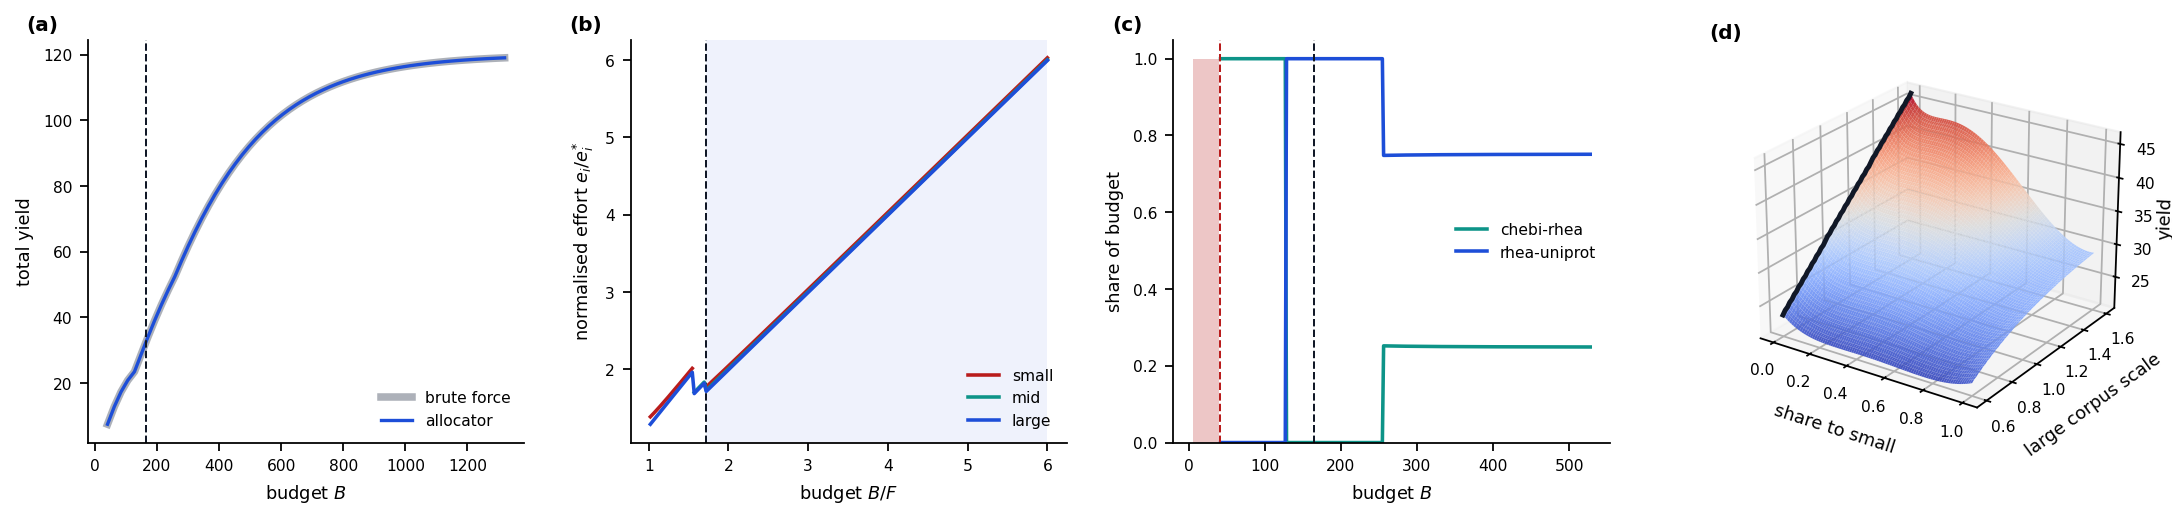
\includegraphics[width=\textwidth]{figures/panel_03_allocator.png}
    \caption{\textbf{The Gated Allocator Against Exhaustive Search.}
    (\textbf{A})~Allocator yield and brute-force yield against budget for the ChEBI--Rhea/Rhea--UniProt pair ($N = 30$ and $90$, so $e^{*}_1 = 40.89$, $e^{*}_2 = 124.07$, $F = \sum_i e^{*}_i = 164.96$). The two curves are visually indistinguishable across the full range; the worst relative gap over $60$ budgets is $9.3 \times 10^{-7}$, which is the resolution of the $800$-step brute-force grid rather than allocator error. The dashed line marks $B = F$.
    (\textbf{B})~Normalised efforts $e_i/e^{*}_i$ against budget $B/F$ for three unequal corpora $\{20, 60, 200\}$ ($e^{*} = 27.03,\,82.48,\,276.57$; $F = 386.07$). Within the shaded water-fill regime, which begins at $B/F = 1.72$, the three converge to a common value---at $B/F = 6$ they are $6.030$, $6.004$ and $5.996$, agreeing to $0.03$ despite raw efforts differing by an order of magnitude. To the left of the shaded band a source receiving nothing is drawn as a \emph{gap} rather than as zero, because there it is unfunded by design under the commit-subset rule and not an equalisation that failed.
    (\textbf{C})~Share of budget allocated to each source across the three policy regimes. Below $B = e^{*}_{\min} = 40.89$ (red dashed) the allocator refuses outright, shaded in red. Between $e^{*}_{\min}$ and roughly $1.7F$ it commits to a proper subset. Only above that does it water-fill, at which point both shares stabilise.
    (\textbf{D})~Total yield over (share to the small source, scale factor on the large corpus) at a budget just above $F$, with the argmax ridge traced in black. The ridge sits pinned at share $= 0$ across the whole range of corpus scalings: at $B = F$ exactly the marginal-equalising interior solution places both sources precisely at threshold and yields $N_1/4 + N_2/4 = 30$, while funding only the larger source yields $32.629$---$8.76\%$ more. Having every source on its concave branch is necessary for an interior optimum, not sufficient for it.}
    \label{fig:panel3}
\end{figure*}

\subsection{A necessary condition mistaken for a sufficient one}
\label{sec:necessarynotsufficient}

The comparison against drop-one-source corners in
\Cref{def:gated}(1) is not defensive programming. It repairs a real
error, and the error is instructive enough to state as a proposition.

\begin{proposition}[Concave branch is necessary, not sufficient]
\label{prop:notsufficient}
$B\ge\sum_i\estar_i$ places every source on its concave branch, and is
therefore necessary for an interior optimum in which all sources are
funded. It is not sufficient: there exist budgets $B\ge\sum_i\estar_i$
at which the optimum funds a proper subset.
\end{proposition}

\begin{proof}
By construction. Take $N_1=30$, $N_2=90$, so $\estar_1=40.89$,
$\estar_2=124.07$, $F=164.96$. At $B=F$ exactly, the marginal-equalising
interior solution allocates $(\estar_1,\estar_2)$, placing both sources
precisely at threshold; by \Cref{thm:threshold}(iii) its yield is
therefore $N_1/4+N_2/4=30$ exactly. Funding only the larger
source---allocating $(0,\,F)$---yields $32.629$, or $8.76\%$ more.
\end{proof}

\begin{remark}
The interior value in that proof is exactly the quarter-corpus law
summed over sources, which is a useful sanity check on the construction:
$B=\sum_i\estar_i$ is the unique budget at which the water-filling
solution puts \emph{every} source exactly at its inflection, and so
recovers precisely a quarter of every corpus.
\end{remark}

The mechanism is visible in \Cref{fig:panel1}(c). Marginal yield
$\yield'$ does not decrease monotonically; it \emph{rises} to a peak at
$\estar$ and falls thereafter. At $B$ just above $F$ every source sits
barely onto its concave branch, where its marginal yield is still near
that peak. Withdrawing one source entirely then frees enough budget to
push another far up its curve, and the gain outweighs the loss.

The first-order condition cannot detect this, because it compares
interior points and the winner is a corner. This is the same structural
fact as \Cref{thm:reversal}, appearing one level up: the KKT conditions
are sufficient only under concavity of the objective \emph{over the
feasible set}, and the feasible set here includes the faces where a
source is unfunded \citep{boyd2004convex}.

\begin{remark}[Why a self-consistency check would have passed]
\label{rem:selfconsistency}
The broken allocator satisfied its own optimality condition exactly:
marginals were equalised to $10^{-10}$. A test asserting ``the returned
allocation equalises marginal yield'' would have passed. What caught it
was checking against exhaustive search over the simplex---a procedure
sharing no line of reasoning with the allocator. This generalises: an
optimality check is only informative if it is not the optimality
condition the implementation was built from.
\end{remark}

Subset selection in \Cref{def:gated}(2) is likewise by enumeration rather
than by a greedy ratio rule. A greedy rule was tried first and is not
optimal, for the same reason: which subset wins depends on how far the
budget pushes each survivor up its own curve, which is not a function of
any per-source ratio computable before the split is known. Enumeration
over subsets is affordable because a pipeline federates a handful of
sources, not hundreds \citep{cormen2009}.

% ---------------------------------------------------------------------

% ---------------------------------------------------------------------

% =====================================================================
\section{Validation}
\label{sec:validation}
% =====================================================================

\subsection{What the suite can establish, and what it cannot}

Every quantity in this paper is closed-form except where noted, so most
checks are exact evaluations rather than estimates. That removes sampling
error as an explanation for a pass, but it also means a passing check
establishes only that the implementation computes what the formula says.
Three things are done to make the suite capable of failing:

\begin{enumerate}[leftmargin=1.4em,itemsep=2pt]
\item \textbf{Negative controls.} Six of the twenty-one checks assert
that something does \emph{not} happen on well-formed input: that the
allocator does not refuse above threshold; that spreading does \emph{not}
lose above threshold; that the concave branch \emph{does} recover T2.
\item \textbf{Independent cross-checks.} The allocator is compared
against brute-force simplex search, which shares no reasoning with it
(\Cref{rem:selfconsistency}).
\item \textbf{A positive control on the detector.} Coupon-collector
retrieval is analytically concave, so the diminishing-returns detector is
run against it first. A failure there would indicate a broken detector
rather than a finding about the world.
\end{enumerate}

\subsection{Results}

Twenty-one checks across three experiments; all pass.

\begin{table}[t]
\centering
\small
\begin{tabular}{@{}llcc@{}}
\toprule
\textbf{Experiment} & \textbf{Claim checked} & \textbf{Checks} &
\textbf{Neg.\ ctrl.} \\
\midrule
\texttt{exp-a} & \Cref{thm:threshold} --- the threshold & 6 & 3 \\
\texttt{exp-b} & \Cref{thm:reversal}, \Cref{prop:normalised} & 7 & 2 \\
\texttt{exp-c} & \Cref{def:gated}, \Cref{thm:refusal-nonvacuous} & 8 & 1 \\
\midrule
\textbf{total} & & \textbf{21} & \textbf{6} \\
\bottomrule
\end{tabular}
\caption{Validation summary. All 21 checks pass. Experiments run in
dependency order: \texttt{exp-a} finds the threshold, \texttt{exp-b}
shows it flips the optimal policy, \texttt{exp-c} tests the
implementation built on both.}
\label{tab:validation}
\end{table}

Four findings are worth stating beyond the pass count.

\paragraph{The three retrieval regimes separate cleanly.}
Distinct-entity retrieval shows marginal yield falling from $1.000$ to
$0.222$ with $0/59$ second differences exceeding tolerance---the positive
control. Paginated retrieval holds marginal yield at $3.000$ throughout
(ratio $1.000$), and is weakly concave with \emph{all} second differences
zero, which is why concavity alone is the wrong criterion and marginal
\emph{decay} is the right one. Federated joins show $31/59$ second
differences positive beyond tolerance.

\paragraph{The convexity is structural, not statistical.} The closed form
evaluated with no sampling is convex at $54/59$ second differences
(maximum $+0.01234$). No number of trials would have made the sampled
curve concave. This check exists because two earlier failures made the
finding look like an artefact (\Cref{sec:ourerrors}).

\paragraph{The quarter-corpus law holds across two decades of $N$.}
$\estar/(2N\ln2)$ rises from $0.949$ to $0.999$ over $N=10\ldots1000$,
and $\yield(\estar)=N/4$ at every $N$ tested, to machine precision.

\paragraph{The allocator matches brute force.} Over budgets from $F$ to
$8F$ the worst relative gap against a $600$-step exhaustive search is
$0.0000\%$; at three unequal sources with a $140$-step search it is
$1.4\times10^{-6}$ (in the allocator's favour, i.e.\ within the search
grid's resolution). Both figures are reported as measured rather than
rounded to zero.

\begin{figure*}[!htbp]
    \centering
    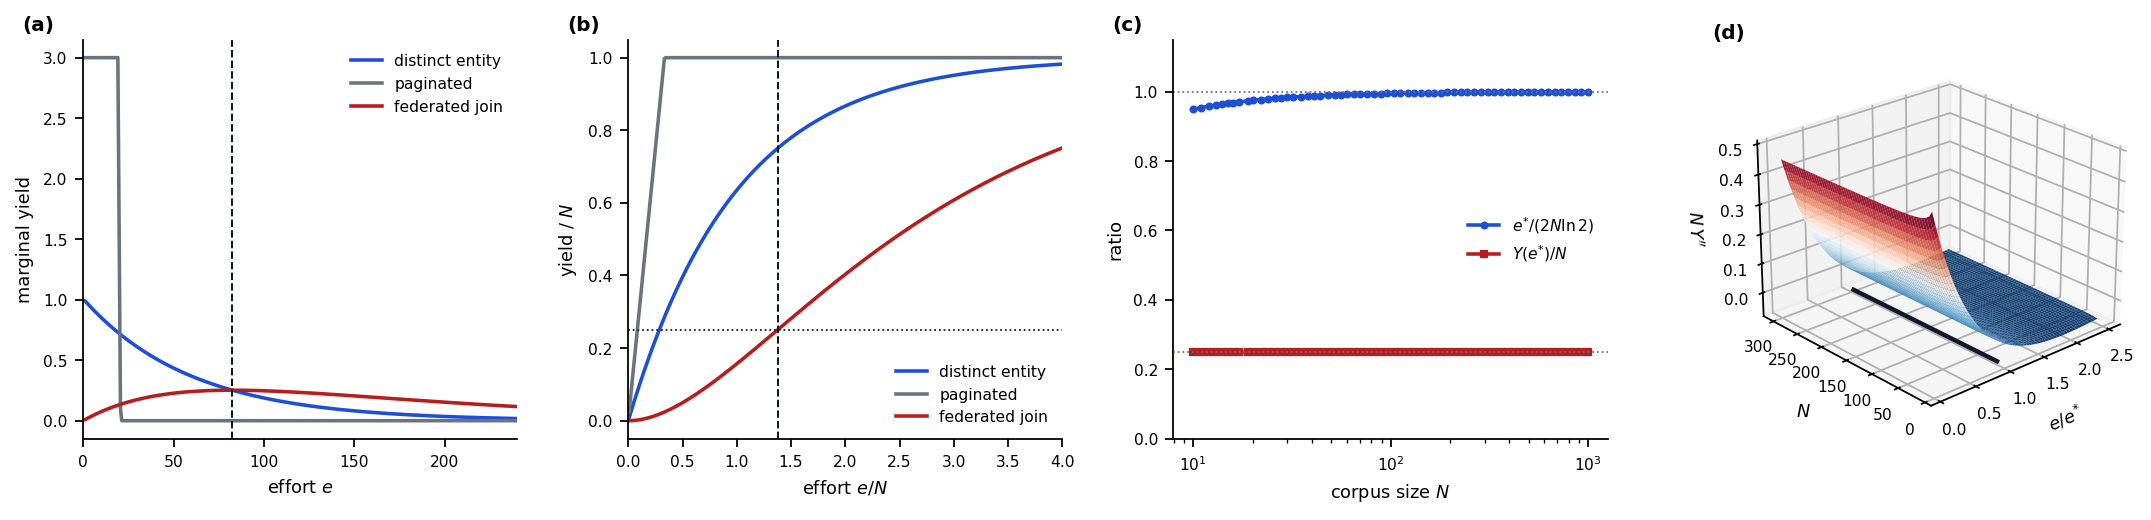
\includegraphics[width=\textwidth]{figures/panel_04_regimes.png}
    \caption{\textbf{Three Retrieval Regimes, and Two Constants Independent of Corpus Size.}
    (\textbf{A})~Marginal yield against effort for three retrieval regimes on common axes at $N = 60$ ($e^{*} = 82.48$, dashed). Distinct-entity retrieval follows coupon-collector coverage $N(1 - (1-1/N)^e)$ and falls monotonically. Paginated retrieval is flat at the page size until the corpus is exhausted, then zero. The federated join alone \emph{rises} to a peak at $e^{*}$ before falling. Only the join violates diminishing returns, and it does so across the entire sub-threshold range---so the assumption underpinning water-filling is environmental rather than structural, and it fails in precisely the environment a federated pipeline operates in.
    (\textbf{B})~The same three regimes as cumulative normalised yield $Y/N$ against $e/N$. The dotted line at $0.25$ and the dashed line at $e^{*}/N = 1.375$ intersect on the join curve, which is the quarter-corpus law located on the same axes as its two controls.
    (\textbf{C})~Two ratios against corpus size on a logarithmic axis, $N$ from $10$ to $10^{3}$. The asymptotic form of the threshold, $e^{*}/(2N\ln 2)$, approaches $1$ from below but is only $0.949$ at $N = 10$ and reaches $0.9995$ at $N = 1000$---an approximation that improves with $N$. The quarter-corpus law $Y(e^{*})/N$ is pinned at $0.25$ to within $3.0 \times 10^{-14}$ at every $N$ tested. One constant is asymptotic; the other is exact.
    (\textbf{D})~Scaled second derivative $N\,Y''$ over $(e/e^{*},\,N)$, red where convex and blue where concave, with the zero contour projected onto the floor. The contour is the plane $e = e^{*}$, flat in $N$: the boundary between increasing and diminishing returns sits at the same normalised effort for every corpus size, which is the threshold theorem rendered as a surface.}
    \label{fig:panel4}
\end{figure*}

\subsection{Two measurement errors and two real ones}
\label{sec:ourerrors}

The medium-vertex paper reports a failing check that became
Proposition~7.1 \citep{sachikonye2026medium}. The same discipline applies
here, and four episodes are worth recording because each changed what we
believed.

\paragraph{Monte Carlo noise five times the signal.} The first attempt to
observe convexity sampled the join process directly. At the trial count
used, the sampling standard error on each second difference exceeded the
true curvature by roughly a factor of five, and the arm failed. The
correct response was not more trials---which we did try---but the
realisation that the question was answerable exactly.

\paragraph{A parity artefact.} The second attempt split effort between
the two sides using an alternating rule indexed by the sample number.
This introduced a period-two component into the yield curve, and the
second-difference detector reported convexity at alternating indices
$[0,2,4,6,8,9]$, a pattern with no physical meaning. A diagnostic
comparing parity, random and analytic splitters showed the analytic
curve---zero noise, no splitter at all---convex at $54/59$ points. That
settled it, and \Cref{cor:structural} is the statement we should have
started from.

\begin{figure*}[!htbp]
    \centering
    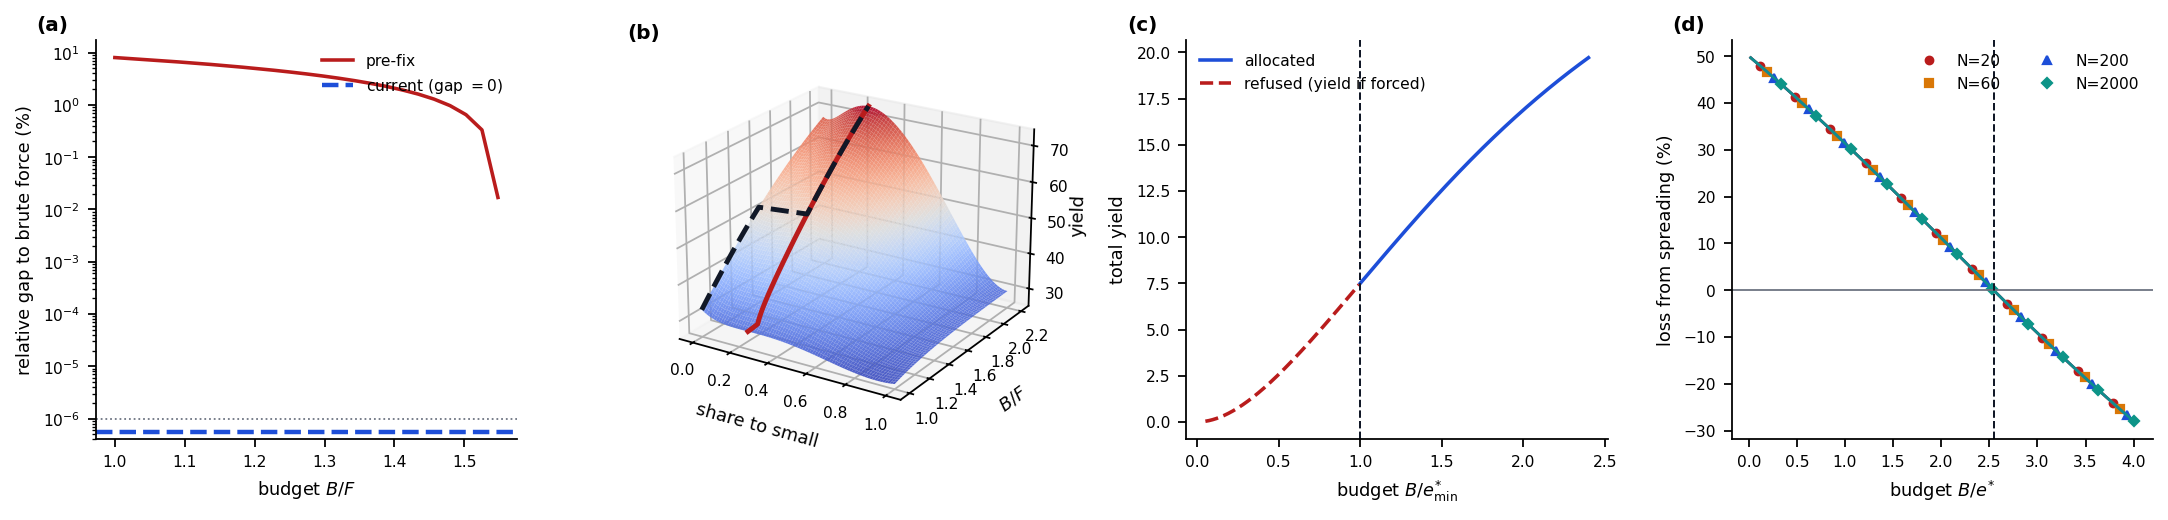
\includegraphics[width=\textwidth]{figures/panel_05_flaw_and_refusal.png}
    \caption{\textbf{An Allocator Flaw Caught by Brute Force, and the Refusal.}
    (\textbf{A})~Relative shortfall against exhaustive search, on a logarithmic axis, for the pre-fix allocation rule (water-fill whenever $B \geq F$) and for the shipped gated rule, over $220$ budgets from $F$ to $6F$. The pre-fix rule is suboptimal at $25$ of them, forfeiting up to $8.0566\%$ of the achievable yield at $B = F$ and recovering only past $B = 1.548F$. The gated allocator's shortfall is identically zero at every budget, so it has no curve to plot and is marked on the floor instead. A self-consistency check would have passed the broken rule; only comparison against a search sharing none of its reasoning exposed it.
    (\textbf{B})~The two allocations traced across the yield surface for $B/F \in [1.0, 2.2]$. The pre-fix interior solution (solid red) sits below the corner the gated rule selects (dashed black) precisely over the region where the surface is still convex, and the two merge once the budget is large enough that the interior solution is genuinely optimal.
    (\textbf{C})~Total yield against budget in units of $e^{*}_{\min} = 40.89$. Below $e^{*}_{\min}$ the allocator refuses to answer; the dashed red continuation is the yield it would have reported had it been forced to. The refusal is not a failure to compute---the number exists---but a statement that no allocation over these sources at this budget is defensible, computable from corpus size alone.
    (\textbf{D})~Loss from spreading rather than committing, against $B/e^{*}$, for four corpus sizes spanning two orders of magnitude ($N = 20, 60, 200, 2000$; markers offset along each curve so the overlap is visible). The four curves coincide to $1.3 \times 10^{-11}$ percentage points: in normalised effort $N$ cancels exactly, so the penalty for ignoring the gate is a function of $B/e^{*}$ alone. The loss runs from $49.7\%$ at $B = 0.02\,e^{*}$ through zero at $u^{\dagger} = 2.5431$ (dashed) to $-28.0\%$ at $B = 4e^{*}$, where spreading has become the better policy by the same margin.}
    \label{fig:panel5}
\end{figure*}

\paragraph{The allocator flaw.} \Cref{prop:notsufficient} was not
anticipated. The allocator was written with $B\ge F$ as the water-filling
gate, which is the natural reading of \Cref{thm:threshold} and is wrong.
It was caught by a single check---agreement with brute force---failing at
$8.0566\%$ at one budget while agreeing to $0.000\%$ at every other. That
the discrepancy was budget-dependent is what made it diagnostic rather
than merely alarming.

\paragraph{A theorem with the wrong boundary, caught by its own figure.}
\Cref{thm:reversal} originally asserted that the symmetric split is
optimal once $B\ge2\estar$, reasoning that both sources are then on their
concave branches. Drawing \Cref{fig:panel2}(a)---which computes the
crossover rather than marking a predicted one---put the zero crossing at
$2.5431$, not at the $2$ the theorem claimed. The theorem was wrong: at
$B=2\estar$ exactly, committing beats the even split by $12.5\%$, and the
true boundary is the $N$-independent constant
$\ucross=2\log_2(1+\sqrt2)$ of \eqref{eq:ucross}.

The error is instructive because it is the \emph{same} error as
\Cref{prop:notsufficient}, made a second time in a different place.
Concavity on the region where all sources exceed threshold is necessary
for the interior optimum and not sufficient for it, because the
competing corner solutions lie outside that region. Having identified
that trap for the multi-source allocator, we reproduced it in the
two-source theorem, and the proof passed inspection because every
individual step in it is true---it simply never compared the interior
stationary point against the endpoints. What caught it was insisting
that figures compute their own reference lines instead of drawing the
value the text predicts.

We also record a check that \emph{passed vacuously} and had to be
replaced. An early mixed-corpus test used corpora of $12$ and $300$,
where the optimum happens to lie at $100\%$ to the small join and
therefore coincides with the commit policy. It passed, but it could not
distinguish a genuine per-join rule from ``always commit''. A sweep over
corpus pairs found $30/90$ at budget $327.13$, where the optimum is
strictly interior and strictly beats both naive policies---the case now
reported in \Cref{sec:reversal}. A check that cannot discriminate between
the hypothesis and its competitor is not evidence for it, whatever its
verdict says.



% =====================================================================
\section{Scope}
\label{sec:scope}
% =====================================================================

\Cref{def:source} makes four assumptions, and each bounds the result
differently.

\paragraph{Uniform draws.} Real endpoints return results in an order
correlated with the query, not uniformly at random. Non-uniformity
concentrates coverage on a subpopulation, which raises $p$ early and
lowers it late---sharpening the sigmoid rather than removing it. The
threshold moves; the convex branch does not disappear.

\paragraph{With replacement.} Sampling without replacement makes coverage
rise strictly faster, reaching $p=1/2$ at lower effort. This lowers
$\estar$ and therefore \emph{shrinks} the refusal region. Our threshold
is thus conservative in the direction that matters: it refuses slightly
more often than necessary rather than allocating where it should not.

\paragraph{Independent sides.} If presence on one side correlates with
presence on the other---plausible when both endpoints derive from a
common curation effort \citep{bansal2022rhea}---then
$\Pr[\text{both}]>p^{2}$ and yield is larger than \Cref{eq:yield}. In the
limit of perfect correlation, yield reduces to $Np$, which is concave
everywhere and T2 applies unconditionally. The convex branch is therefore
a consequence of \emph{independence}, and an agent that knows its sources
are correlated should say so.

\paragraph{Even split between sides.} Effort is split evenly. An agent
free to allocate asymmetrically \emph{between} the two sides of one join
has a further optimisation available which we have not characterised. We
expect it to matter most when the two sides have very different
$N$---which \Cref{def:source} excludes by construction, since $N$ counts
keys joinable on both---but we have not measured it.

Two further limits are worth naming. We have not connected the allocator
to the coordination machinery of T1--T7: an agent that refuses one join
should presumably re-offer that budget to its peers, and the conserved
character invariant and Kuramoto coupling
\citep{sachikonye2026splitattention,kuramoto1975} are the natural
mechanism, but we have not built it. And we have not run the allocator
against live endpoints; every number here is closed-form or simulated,
and a corpus size estimated from a count query carries its own error
which we have not propagated.

% =====================================================================
\section{Conclusion}
\label{sec:conclusion}
% =====================================================================

An assumption that a theorem flags as environmental should be measured in
the environment. We measured T2's in federated retrieval and found it
false below an effort threshold that is exact, closed-form, and
computable from a count query: $\estar=2\ln2/\ln(1/(1-1/N))\to 2N\ln2$,
equivalently the point at which a quarter of the joinable corpus has been
recovered. The failure is not a matter of degree. Below the threshold the
optimum is at a corner and water-filling recommends the opposite action,
losing up to $97\%$ of achievable yield, worst for the agents with the
least budget.

What follows is not a repair of T2 but a gate on it. The allocator works
in normalised effort $\eff/\estar$, gates per source rather than
globally, water-fills where the hypothesis holds, commits where it does
not, and refuses where neither is founded---reporting the budget at which
it could proceed. This is the same shape of refusal the medium vertex
supplies to the receiver language \citep{sachikonye2026medium}, arrived
at independently and for the same reason: a system that always returns an
answer has not said anything by returning one.

The methodological residue may be the more portable part. Two of our
three surprises were our own measurement errors, and both initially
looked like findings; the third was a genuine flaw that satisfied the
implementation's own optimality condition exactly and was caught only by
a check that shared no reasoning with it. A suite of checks that an
implementation would pass by construction measures the implementation's
self-consistency, which was never in doubt.

% =====================================================================
\section*{Reproducibility}
% =====================================================================

All experiments are in
\shk{models/publications/attention-allocated-retrieval/validation/}.
Running \shk{python run\_all.py} executes \texttt{exp-a}, \texttt{exp-b}
and \texttt{exp-c} in dependency order, propagates exit codes, and writes
per-experiment JSON together with an aggregate to \shk{results/}. Every
numerical value quoted in this paper is drawn from those files. The
allocator is \shk{validation/kernel/allocator.py}; the brute-force
comparison it is checked against is in \shk{exp\_c\_allocator.py} and is
deliberately written without reference to it.

% =====================================================================
\bibliographystyle{plainnat}
\bibliography{references}

\end{document}
